\section{Results}
We present qualitative and quantitative evaluations of our method, analyzing our spatial and appearance control components separately to isolate their respective effects.

\subsection{Evaluation Setup}
% \subsection{Baselines and Metrics}
This subsection details the evaluation settings for both control modalities.
\paragraph{Spatial Control.}
To evaluate our local spatial control, we compiled a diverse dataset of 27 scenes covering a wide range of object categories. For each scene, we designate distinct high-control ($\tau_i = 10$) and low-control ($\tau_i = 3$) regions. The internal bounding boxes of our method (see Section~\ref{sec:spatial_local_control}) are used to compute part-wise evaluation metrics where appropriate. We compare our performance against the global conditioning approach of SpaceControl, configured with uniform control strengths of either $\tau = 3$ or $\tau = 10$ across the entire asset.

\paragraph{Appearance Control.}
To evaluate local appearance and texture control, we generated a set of $X$ test cases featuring localized texture conditioning. We compare our method against TRELLIS and GuideFlow3D, the two baselines upon which our appearance framework is built.

\subsection{Spatial Control}

\paragraph{Feature Cosine Distance.}
To quantitatively evaluate the behavior of our local spatial control, we define a feature-based metric that measures the deviation of local-$\tau$ assets from a globally controlled reference asset (generated with $\tau_i = 10$ for all primitives, representing strict adherence to the provided spatial control). 

For each active voxel $v$ in the generated asset structure $\mathcal{V}$ with spatial coordinate $\mathbf{x}_v$ and feature representation $\mathbf{f}_v$, we find its nearest spatial neighbor $v^*$ in the reference asset structure $\mathcal{V}^*$:
\begin{equation}
v^* = \arg\min_{u \in \mathcal{V}^*} \|\mathbf{x}_v - \mathbf{x}_u\|_2.
\end{equation}
We then compute the cosine distance between their corresponding PartField feature representations:
\begin{equation}
d_{\text{feat}}(v) = 1 - \frac{\mathbf{f}_v \cdot \mathbf{f}_{v^*}}{\|\mathbf{f}_v\|_2 \|\mathbf{f}_{v^*}\|_2}.
\label{eq:cosine_dist}
\end{equation}

The regional distance metric $D_{\text{region}}$ is computed by averaging $d_{\text{feat}}(v)$ over the subset of voxels $\mathcal{V}_{\text{region}} \subseteq \mathcal{V}$ corresponding to either the high-control or low-control primitives.

Figure~\ref{fig:cosineship} visualizes this metric. Our method closely matches the reference shape in the high-control regions (indicated by low feature distances), while deviating in the low-control regions to generate realistic details aligned with the text prompt (e.g., the hull and sails of a sailboat).

\begin{figure}[t]
    \centering
    \includegraphics[width=0.70\linewidth]{figs/shipcosine.pdf}
    \caption{\textbf{Visualization of feature cosine distance.} Left: Input superquadrics (top, orange: high-control, gray: low-control) and the \methodname asset (bottom). Right: Voxel-wise cosine distance between the generated asset's features and the nearest spatial match in the globally controlled ($\tau = 10$) reference.}
    \label{fig:cosineship}
\end{figure}

Figure~\ref{fig:control_regions_distance} reports the average cosine distance across our test set. The results show a $74\%$ increase in the mean feature distance within the low-control regions compared to the high-control regions ($\Delta = 0.18$). This confirms that our method successfully grants generative freedom in low-control areas to produce plausible details while maintaining stricter control in designated high-control regions.

\begin{figure}[t]
\centering
\begin{tikzpicture}
\begin{axis}[
  width=\columnwidth,
  height=0.38\columnwidth,
  xmin=0,
  xmax=0.5,
  ymin=-0.32,
  ymax=1.45,
  clip=false,
  axis x line*=bottom,
  axis y line=none,
  tick style={black, line width=0.5pt},
  xtick={0,0.1,0.2,0.3,0.4,0.5},
  xticklabels={0,0.1,0.2,0.3,0.4,0.5},
  xticklabel style={font=\footnotesize},
  ytick=\empty,
  xmajorgrids=true,
  major grid style={draw=gray!22, line width=0.45pt},
]

% High-control line
\addplot[
  highblue,
  line width=3.2pt,
  line cap=round
] coordinates {(0,1) (0.24,1)};

\addplot[
  only marks,
  mark=*,
  mark size=5.0pt,
  draw=highblue,
  fill=highblue
] coordinates {(0.24,1)};

% Low-control line
\addplot[
  loworange,
  line width=3.2pt,
  line cap=round
] coordinates {(0,0) (0.42,0)};

\addplot[
  only marks,
  mark=*,
  mark size=5.0pt,
  draw=loworange,
  fill=loworange
] coordinates {(0.42,0)};
% Value labels
\node[
  font=\footnotesize,
  anchor=west,
  fill=white,
  inner sep=0.7pt
] at (axis cs:0.252,1.03) {$0.24$};

\node[
  font=\footnotesize,
  anchor=west,
  fill=white,
  inner sep=0.7pt
] at (axis cs:0.432,-0.02) {$0.42$};

% Delta bracket
\draw[
  deltapurple,
  line width=0.85pt
] (axis cs:0.24,0.40) -- (axis cs:0.42,0.40);

\draw[
  deltapurple,
  line width=0.85pt
] (axis cs:0.24,0.35) -- (axis cs:0.24,0.48);

\draw[
  deltapurple,
  line width=0.85pt
] (axis cs:0.42,0.35) -- (axis cs:0.42,0.48);

\node[
  font=\scriptsize,
  anchor=south,
  fill=white,
  inner sep=1pt
] at (axis cs:0.33,0.46)
{$\Delta=0.18$ {\tiny$(+74\%)$}};

\end{axis}
\end{tikzpicture}
\caption{Mean cosine distance to the globally controlled reference ($\tau=10$) in the PartField feature space, comparing high-control (blue) and low-control (orange) regions over the assets of our test set.
\vspace{-4mm}}
\label{fig:control_regions_distance}
\end{figure}

\paragraph{Geometric and Textual Alignment.}
In addition to evaluating local feature-level variations, we assess the overall geometric precision and semantic alignment of our method using standard 3D generation metrics. Specifically, to measure spatial adherence to the input superquadrics, we compute the Chamfer Distance (CD) separately on the designated high-control ($CD_{\text{high}}$) and low-control ($CD_{\text{low}}$) regions. A lower $CD_{\text{high}}$ indicates closer compliance with the user's spatial constraints, whereas a higher $CD_{\text{low}}$ indicates that the model has the geometric freedom to reinterpret and detail the low-control regions. To evaluate semantic alignment, we compute the CLIP text distance between the rendered assets and the input prompts.

Table~\ref{tab:quantitative_spatial} presents the quantitative comparison between our local-$\tau$ method and two global baselines: $\tau = 3$ (weak global control) and $\tau = 10$ (strong global control). In the low-control regions, our method achieves a $CD_{\text{low}}$ of $11.39$, matching the flexibility of the weak baseline ($\tau = 3$). On the other hand, in the high-control regions, our method achieves a low error of $2.44$, closely approaching the strict compliance of the strong baseline ($\tau = 10$).

Furthermore, our CLIP text-alignment score ($0.243$) is comparable to both baselines. This demonstrates that introducing localized, variable control strengths does not degrade the prompt-following capabilities of the underlying model.

\begin{table}[t]
\centering
\small
\begin{tabular}{lccc}
\toprule
Method & $CD_{\text{high}} \downarrow$ & $CD_{\text{low}} \uparrow$ & CLIP-text $\downarrow$ \\
\midrule
$\tau=3$ & 9.29 $\pm$ 7.46 & 11.28 $\pm$ 13.95 & 0.247 $\pm$ 0.020 \\
local-$\tau$ & 2.44 $\pm$ 1.55 & 11.39 $\pm$ 17.32 & 0.243 $\pm$ 0.017 \\
$\tau=10$ & 0.87 $\pm$ 0.51 & 2.73 $\pm$ 5.51 & 0.235 $\pm$ 0.019 \\
\bottomrule
\end{tabular}
\caption{\textbf{Quantitative evaluation of spatial control and prompt alignment.} We report Chamfer Distance (CD) on high-control regions ($CD_{\text{high}} \downarrow$) and low-control regions ($CD_{\text{low}} \uparrow$), alongside CLIP text-image distance (CLIP-text $\downarrow$). Our local-$\tau$ control achieves strict geometric compliance in high-control areas (low $CD_{\text{high}}$) while matching the generative freedom of $\tau = 3$ in low-control areas (high $CD_{\text{low}}$), without compromising semantic alignment.}
\label{tab:quantitative_spatial}
\end{table}

\paragraph{User study.}
%In addition to geometric and feature space metrics, we conducted a pairwise user study for perceptual evaluation of the generated assets. Our local-$\tau$ control was compared against two global $\tau$ baselines, $\tau=3$ and $\tau=10$. For each of 19 test scenes we generated three outputs with local or global conditioning from the same superquadric inputs and prompts, and asked participants to compare local-$\tau$ against each baseline separately. Shown two outputs side by side as interactive 3D models, participants indicated which output followed the high- and low-control input superquadrics at the desired level of control, which looked more realistic and which they preferred overall. The study encompassed 39 individuals and 333 trials in total.

To complement our quantitative metrics, we conducted a pairwise user study evaluating the perceptual quality of the generated assets. We compared our local-$\tau$ control against uniform global baselines of $\tau = 3$ and $\tau = 10$. Using 19 test scenes, we generated three outputs (local-$\tau$, $\tau=3$, and $\tau=10$) from identical prompts and superquadric inputs. Participants viewed interactive 3D model pairs side-by-side and evaluated them based on shape fidelity, realism, and overall preference. The study collected 333 trials from 39 participants.

%Figure \ref{fig:user_study_local_tau} reports the resulting win/tie/loss rates. Against $\tau=3$, local-$\tau$ is preferred on shape fidelity in 81\% of comparisons, while remaining comparable on realism (47\% wins, 16\% ties) and overall preference (50\% wins, 15\% ties). Against $\tau=10$, local-$\tau$ is judged more realistic in 74\% of comparisons and preferred overall in 70\%. On shape fidelity, however, its win rate against $\tau=10$ drops to 37\%. We suspect this reflects how participants interpreted the question, which asked which object better matches the prompt in the low-control region while also following the input shape in the high-control region. Since $\tau=10$ follows the input shape closely everywhere, including the low-control region, participants may have judged overall resemblance to the input shape rather than distinguishing between the two regions. 

% Across both comparisons, local-$\tau$ conditioning avoids the trade-off that uniform control enforces on the entire object. Rather than fixing one global setting between fidelity and realism, it resolves that trade-off separately for each region of the asset. 


As shown in Fig.~\ref{fig:user_study_local_tau}, local-$\tau$ is preferred for shape fidelity in $81\%$ of comparisons against $\tau=3$, while achieving comparable results for realism ($47\%$ wins, $16\%$ ties) and overall preference ($50\%$ wins, $15\%$ ties). Against the higher control global baseline ($\tau=10$), local-$\tau$ is judged significantly more realistic ($74\%$ wins) and is preferred overall ($70\%$ wins). On shape fidelity, its win rate against $\tau=10$ falls to $37\%$. We attribute this to participants prioritizing overall resemblance to the input shape (which $\tau=10$ enforces globally) rather than evaluating only the high control region as requested. Overall, local-$\tau$ conditioning avoids the trade-off that uniform control enforces on the entire object. Rather than fixing one global setting between fidelity and realism, it resolves that trade-off separately for each region of the asset. 



%userstudy
% user study
\begin{figure}[t]
\centering
\resizebox{\columnwidth}{!}{%
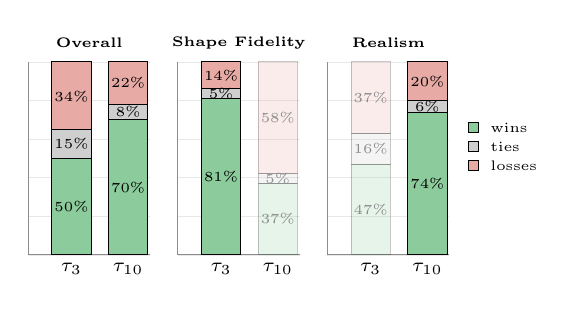
\begin{tikzpicture}

% ---------- colors ----------
\definecolor{wincol}{HTML}{8CCB9B}
\definecolor{tiecol}{HTML}{CFCFCF}
\definecolor{losscol}{HTML}{E7AAA5}

% ---------- dimensions ----------
\def\H{2.45}
\def\barw{0.5}
\def\xA{0.30}
\def\xB{1.02}
\def\panelw{1.55}

% ---------- panel macro ----------
\newcommand{\drawpanel}[3]{%
  % #1 = x offset, #2 = title, #3 = y labels? 1/0

  % grid
  \foreach \p in {0,20,40,60,80,100} {
    \pgfmathsetmacro{\yy}{\p*\H/100}
    \draw[gray!18, line width=0.25pt]
      ({#1},\yy) -- ({#1+\panelw},\yy);
  }

  % axes
  \draw[black!45, line width=0.35pt] ({#1},0) -- ({#1+\panelw},0);
  \draw[black!45, line width=0.35pt] ({#1},0) -- ({#1},\H);

  % y labels, no percent signs
  %\ifnum#3=1
    %\foreach \p in {0,20,40,60,80,100} {
     % \pgfmathsetmacro{\yy}{\p*\H/100}
     % \node[anchor=east, font=\tiny] at ({#1-0.04},\yy) {\p};
   % }
  %\fi

  % title
  \node[font=\bfseries\tiny, align=center]
    at ({#1+\panelw/2},{\H+0.24}) {#2};
}

% ---------- stacked bar macro ----------
\newcommand{\stackbar}[7]{%
  % #1 = x
  % #2 = wins
  % #3 = ties
  % #4 = losses
  % #5 = opacity
  % #6 = label color
  % #7 = show labels? 1/0

  \pgfmathsetmacro{\yw}{#2*\H/100}
  \pgfmathsetmacro{\yt}{#3*\H/100}
  \pgfmathsetmacro{\yl}{#4*\H/100}

  % wins
  \draw[
    fill=wincol,
    fill opacity=#5,
    draw=black,
    draw opacity=#5,
    line width=0.35pt
  ] (#1,0) rectangle ({#1+\barw},{\yw});

  % ties
  \draw[
    fill=tiecol,
    fill opacity=#5,
    draw=black,
    draw opacity=#5,
    line width=0.35pt
  ] (#1,\yw) rectangle ({#1+\barw},{\yw+\yt});

  % losses
  \draw[
    fill=losscol,
    fill opacity=#5,
    draw=black,
    draw opacity=#5,
    line width=0.35pt
  ] (#1,{\yw+\yt}) rectangle ({#1+\barw},\H);


  \ifnum#7=1
    \node[font=\tiny, text=#6]
      at ({#1+\barw/2},{\yw/2}) {#2\%};

    \node[font=\tiny, text=#6]
      at ({#1+\barw/2},{\yw+\yt/2}) {#3\%};

    \node[font=\tiny, text=#6]
      at ({#1+\barw/2},{\yw+\yt+\yl/2}) {#4\%};
  \fi
  

}

% ==================================================
% Overall
% ==================================================
\drawpanel{0}{Overall}{1}
\stackbar{0+\xA}{50}{15}{34}{1.0}{black}{1}
\stackbar{0+\xB}{70}{8}{22}{1.0}{black}{1}
\node[font=\scriptsize] at ({0+\xA+\barw/2},-0.18) {$\tau_{3}$};
\node[font=\scriptsize] at ({0+\xB+\barw/2},-0.18) {$\tau_{10}$};

% ==================================================
% Shape fidelity
% ==================================================
\drawpanel{1.90}{Shape Fidelity}{0}
\stackbar{1.90+\xA}{81}{5}{14}{1.0}{black}{1}
\stackbar{1.90+\xB}{37}{5}{58}{0.22}{black!45}{1}
\node[font=\scriptsize] at ({1.90+\xA+\barw/2},-0.18) {$\tau_{3}$};
\node[font=\scriptsize] at ({1.90+\xB+\barw/2},-0.18) {$\tau_{10}$};

% ==================================================
% Realism
% ==================================================
\drawpanel{3.80}{Realism}{0}
\stackbar{3.80+\xA}{47}{16}{37}{0.22}{black!45}{1}
\stackbar{3.80+\xB}{74}{6}{20}{1.0}{black}{1}
\node[font=\scriptsize] at ({3.80+\xA+\barw/2},-0.18) {$\tau_{3}$};
\node[font=\scriptsize] at ({3.80+\xB+\barw/2},-0.18) {$\tau_{10}$};

% ==================================================
% Compact legend
% ==================================================
\begin{scope}[shift={(5.72,1.55)}]
  \draw[fill=wincol, draw=black, line width=0.3pt] (-0.13,0.00) rectangle (0,0.13);
  \node[anchor=west, font=\tiny] at (0.03,0.065) {wins};

  \draw[fill=tiecol, draw=black, line width=0.3pt] (-0.13,-0.24) rectangle (0,-0.11);
  \node[anchor=west, font=\tiny] at (0.03,-0.175) {ties};

  \draw[fill=losscol, draw=black, line width=0.3pt] (-0.13,-0.48) rectangle (0,-0.35);
  \node[anchor=west, font=\tiny] at (0.03,-0.415) {losses};
\end{scope}

\end{tikzpicture}
}

\caption{User study comparing \methodname against fixed $\tau$ baselines. Dimmed bars show non-primary comparisons.}
\label{fig:user_study_local_tau}

\end{figure}


\subsection{Appearance Control}

\subsection{Joint Control}

\subsection{Ablations}